%%%%%%%%%%%%%%%%%%%%%%%%%%%%%%%%%%%%%%%%%%%%%%%%%%%%%%%%%%%%%%%%%%%%%%%%%%%

\documentclass{standalone}

\usepackage{amsmath}
\usepackage{mathptmx}
\usepackage{pgfplots}
\usetikzlibrary{external}
\tikzexternalize{hinoki-cypress-linear}
\pgfplotsset{compat=1.16}

%% IEEE uses Times Roman font, so we'll default to Times.
%% These three commands make up the entire times.sty package.
\renewcommand{\rmdefault}{ptm}
\renewcommand{\ttdefault}{pcr}
\normalfont\selectfont

\begin{document}

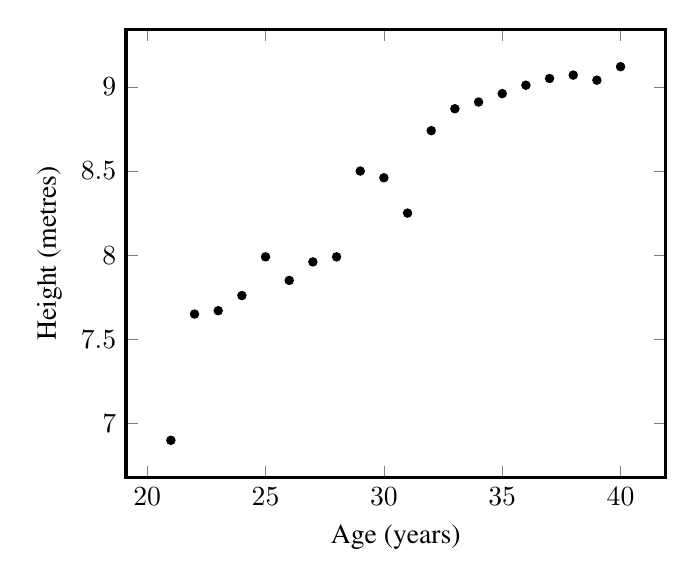
\begin{tikzpicture}
\tikzset{%%
  every mark/.append style={scale=1.0},%%
  scale=1.0%%
}
\pgfplotsset{%%
  every axis/.append style={font=\normalsize}%%
}
%%
\begin{axis}[%%
  axis line style=very thick,%%
  dotStyle/.style={mark size=1.5,black,mark color=black,mark=*,only marks},%%
  enlargelimits=true,%%
  %% x axis
  xlabel={\normalsize Age (years)},%%
  %% y axis
  ylabel={\normalsize Height (metres)}%%
]
%%
%%
\addplot[dotStyle] coordinates {
  (21, 6.9)
  (22, 7.65)
  (23, 7.67)
  (24, 7.76)
  (25, 7.99)
  (26, 7.85)
  (27, 7.96)
  (28, 7.99)
  (29, 8.5)
  (30, 8.46)
  (31, 8.25)
  (32, 8.74)
  (33, 8.87)
  (34, 8.91)
  (35, 8.96)
  (36, 9.01)
  (37, 9.05)
  (38, 9.07)
  (39, 9.04)
  (40, 9.12)
};
\end{axis}
\end{tikzpicture}

\end{document}
